\subsection{Project Management}

In this section, we will be explaining how we have maintained part-1 and part-2 of the project using GitHub. We have used the concept of branches, issues, pull requests, and Kanban board using GitHub projects to track and maintain progress throughout the project.

\subsubsection{GitHub Project Repository}

We have maintained our entire project using the following GitHub repository:

\url{https://github.com/abhinavcreed13/project-space-optimisation-group-3}

This repository was kept private and the access was shared with our supervisor Prashant Madumal (@prashanm) and our client Anbin Hou (@anbinhou). With the approval of our client, we have deleted the sensitive data and repository is made public for evaluation purposes.

\begin{figure}[H]
\centering
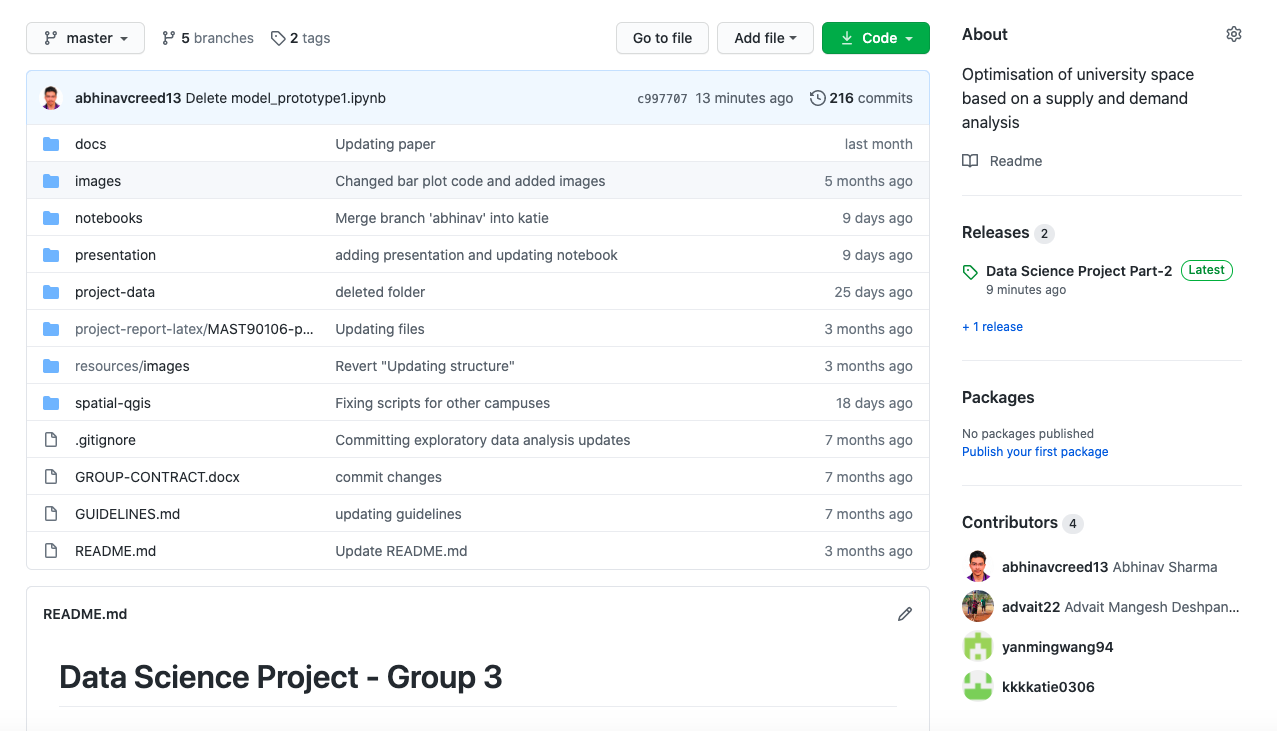
\includegraphics[width=16cm]{resources/images/github/github1.png}
\caption{Project's GitHub Repository with tagged releases}
\label{fig:github1}
\end{figure}

The code and contributions in this repository are maintained using the concept of branching which is heavily used in this project as shown in the figure below.

\begin{figure}[H]
\centering
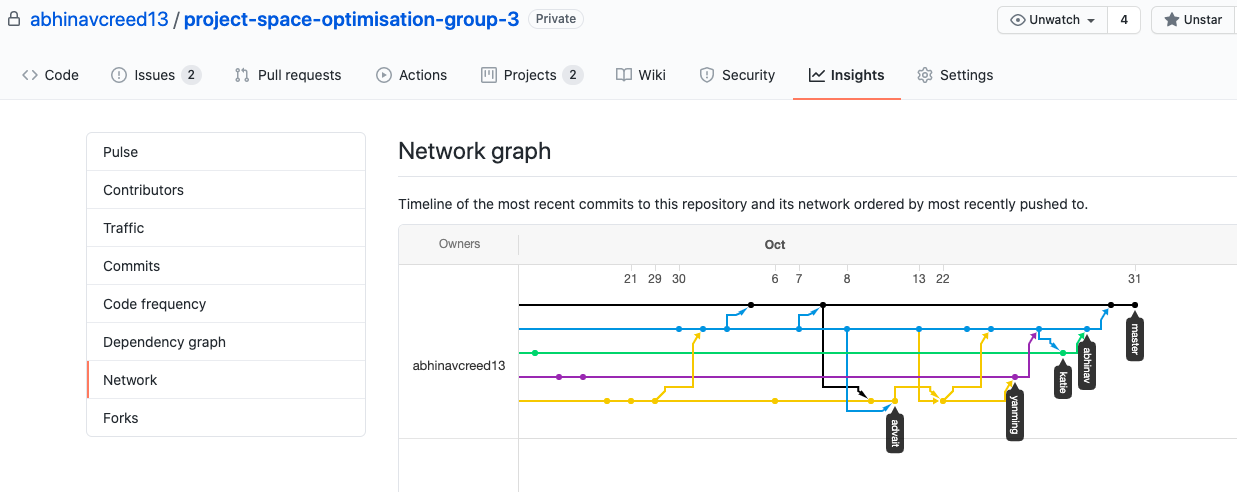
\includegraphics[width=16cm]{resources/images/github/github2.png}
\caption{GitHub branching concept for effective work distribution and contribution}
\label{fig:github2}
\end{figure}

These individual person's branches are effectively merged across each other throughout the project to keep progress in sync using the pull requests feature of GitHub as shown in the figure below.

\begin{figure}[H]
\centering
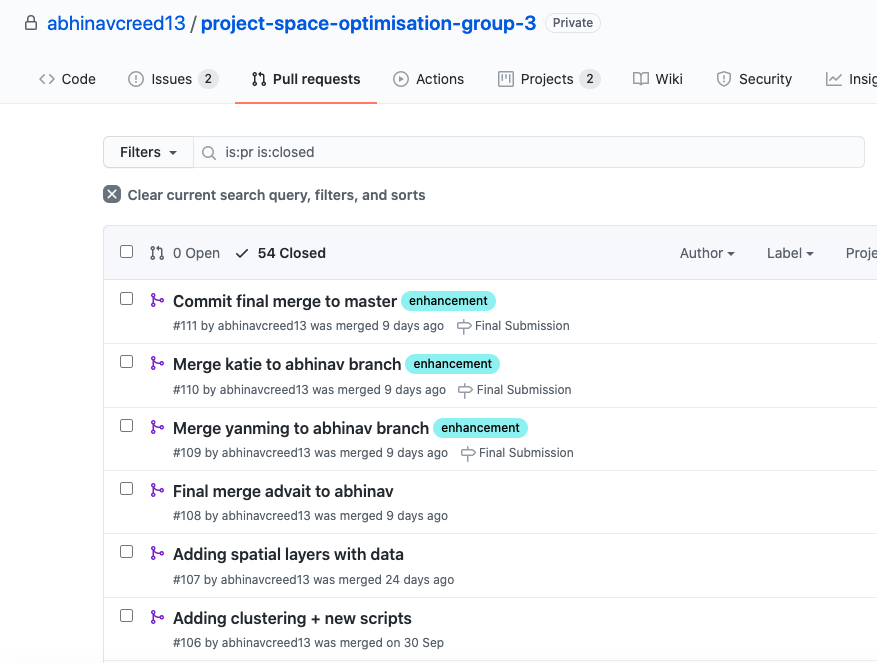
\includegraphics[width=12cm]{resources/images/github/github3.png}
\caption{GitHub pull requests used for syncing branches}
\label{fig:github3}
\end{figure}

\subsubsection{GitHub Project Tracking}

In order to track the progress of our team in the project, we used several inbuilt features of the GitHub. First, we created several milestones throughout the part-1 and part-2 of the project and assigned issues to the corresponding milestones for effective tracking of the progress. A snapshot of the recent milestones is shown in the figure below.

\begin{figure}[H]
\centering
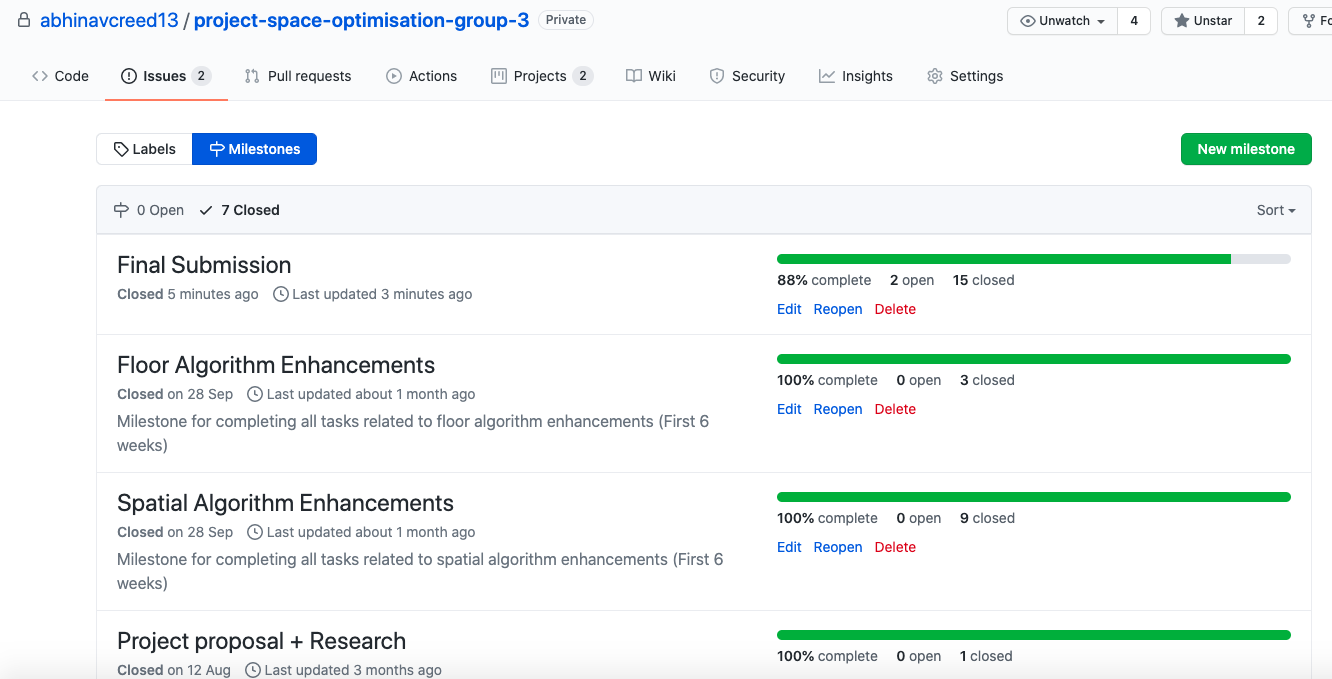
\includegraphics[width=12cm]{resources/images/github/github4.png}
\caption{GitHub milestones for tracking progress}
\label{fig:github4}
\end{figure}

These milestones are connected with their corresponding issues that are assigned to the team members so that their contribution and progress can be tracked. A snapshot of the closed issues is shown in the figure below.

\begin{figure}[H]
\centering
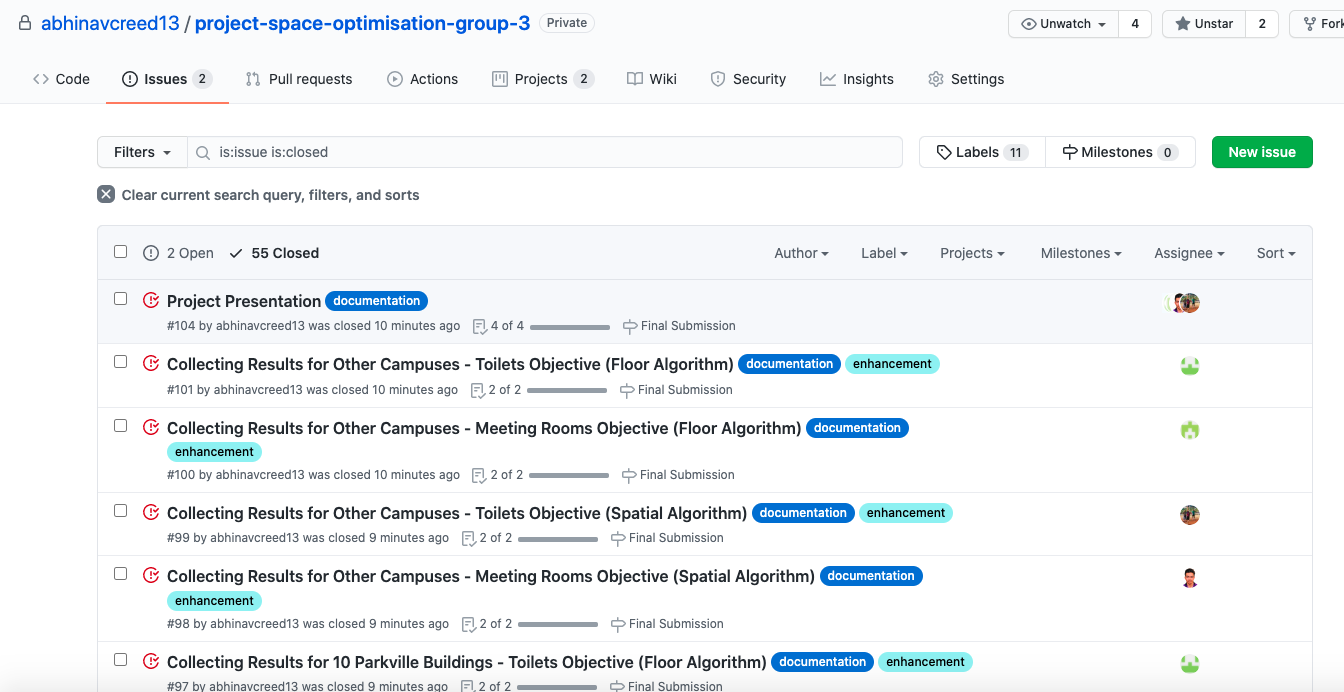
\includegraphics[width=12cm]{resources/images/github/github5.png}
\caption{GitHub issues feature for assigning tasks to the team-mates}
\label{fig:github5}
\end{figure}

In order to effectively manage these issues and their corresponding status, we have also used the GitHub projects feature where we can track all the issues and pull requests collectively as shown in the figure below.

\begin{figure}[H]
\centering
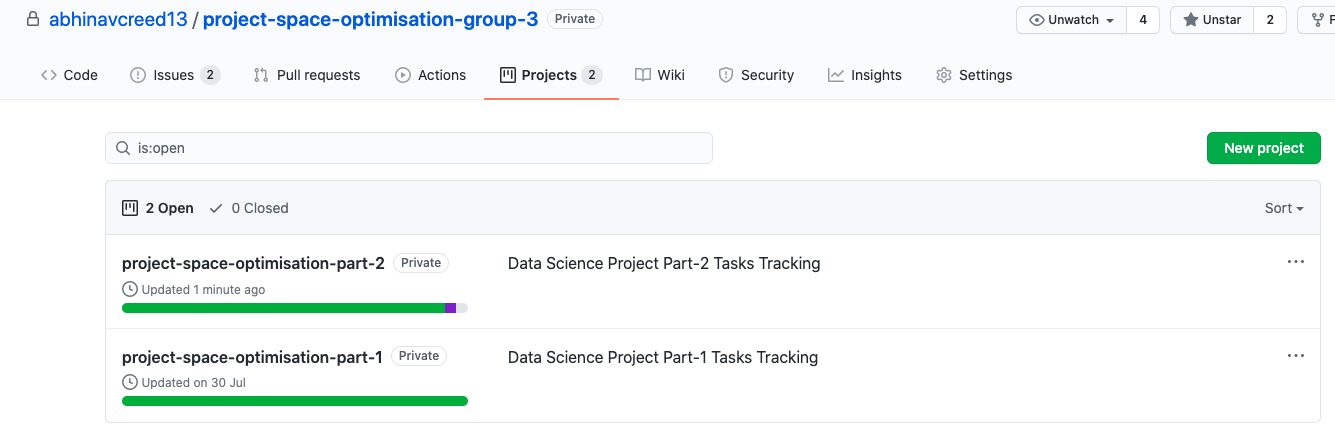
\includegraphics[width=12cm]{resources/images/github/github6.png}
\caption{GitHub projects for part-1 and part-2}
\label{fig:github6}
\end{figure}

Finally, these projects are effectively used with the kanban board to view the tasks that are required to be picked by the teammate, tasks that are in progress, and tasks that are already completed. These board-based tracking helped us a lot in effectively viewing the progress of the project and showing this progress to our supervisor and the client. A snapshot of our project's part-2 kanban board is shown in the figure below.

\begin{figure}[H]
\centering
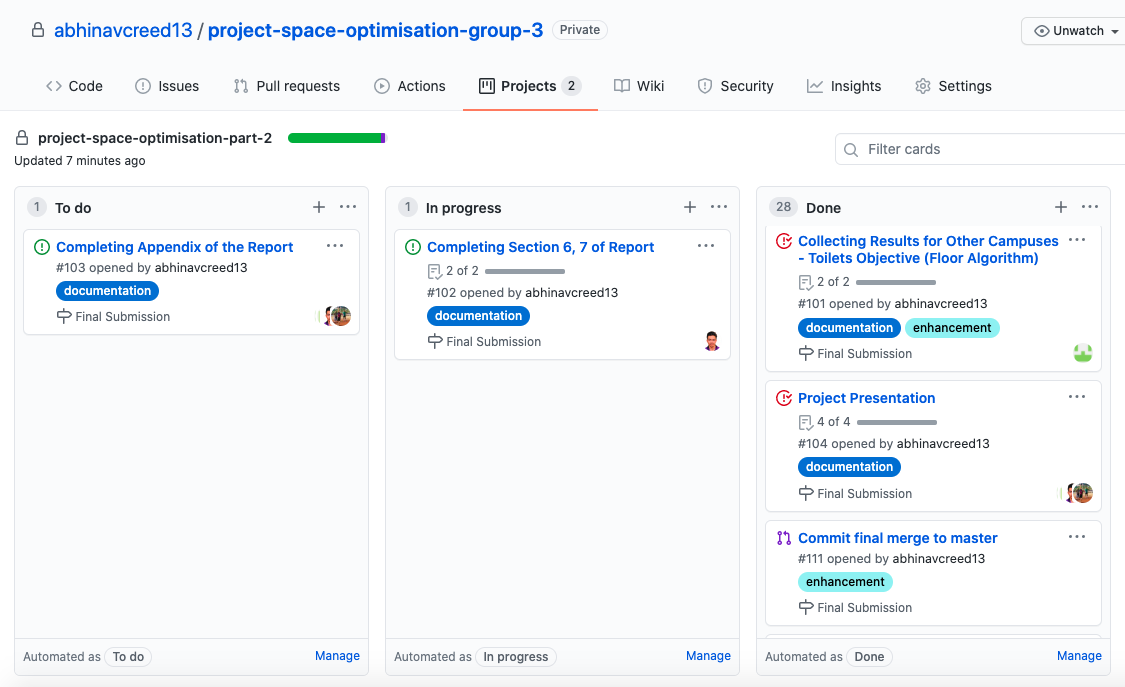
\includegraphics[width=14cm]{resources/images/github/github7.png}
\caption{GitHub project part-2 kanban board}
\label{fig:github7}
\end{figure}

\subsubsection{Client \& Supervisor Meeting Logs}

In this section, we will be showing complete meeting logs with our client and supervisor for both part-1 and part-2 of the project. We will also show the meeting timings with their corresponding agenda.

\paragraph{Data Science Project Part-1 Logs}

\begin{table}[H]
\resizebox{\textwidth}{!}{
\begin{tabular}{|l|l|l|l|}
\hline
\textbf{Meeting Week} & \textbf{Meeting Date \& Time} & \textbf{Meeting Hosts}                                                                                         & \textbf{Meeting Agenda}                                                                                                                 \\ \hline
Week 4                & 3/27/2020, 3:00 - 4:00 PM     & \begin{tabular}[c]{@{}l@{}}Jade Germantis (Client)\\ Anbin Hou (Client)\\ Prashan Madumal (Super)\end{tabular} & \begin{tabular}[c]{@{}l@{}}- First meeting with the client\\ - Project introduction\end{tabular}                                        \\ \hline
Week 5                & 4/4/2020, 10:00 - 11:00 AM    & Prashan Madumal (Super)                                                                                        & \begin{tabular}[c]{@{}l@{}}- First meeting with the supervisor\\ - Project plan discussion\end{tabular}                                 \\ \hline
Week 6                & 4/21/2020 , 12:00 - 1:00 PM   & \begin{tabular}[c]{@{}l@{}}Anbin Hou (Client)\\ Prashan Madumal (Super)\end{tabular}                           & \begin{tabular}[c]{@{}l@{}}- Project data-based questions with client\\ - Supply Demand Correlations Analysis presentation\end{tabular} \\ \hline
Week 6                & 4/24/2020, 10:00 - 11:00 AM   & Prashan Madumal (Super)                                                                                        & \begin{tabular}[c]{@{}l@{}}- Report discussion\\ - Data Analysis progress presentation\end{tabular}                                     \\ \hline
Week 7                & 5/1/2020, 10:00 - 11:00 AM    & Prashan Madumal (Super)                                                                                        & \begin{tabular}[c]{@{}l@{}}- EDA progress\\ - Correlation analysis progress\end{tabular}                                                \\ \hline
Week 8                & 5/8/2020, 10:00 - 11:00 AM    & Prashan Madumal (Super)                                                                                        & \begin{tabular}[c]{@{}l@{}}- Spatial data analysis progress\\ - Data preprocessing discussion\end{tabular}                              \\ \hline
Week 9                & 5/15/2020, 10:00 - 11:00 AM   & Prashan Madumal (Super)                                                                                        & - Client meeting presentation discussion                                                                                                \\ \hline
Week 9                & 5/15/2020, 3:15 - 4:15 PM     & \begin{tabular}[c]{@{}l@{}}Anbin Hou (Client)\\ Prashan Madumal (Super)\end{tabular}                           & \begin{tabular}[c]{@{}l@{}}- Spatial data analysis QGIS 3 showcase\\ - Floor prediction model showcase\end{tabular}                     \\ \hline
Week 10               & 5/22/2020, 10:00 - 11:00 AM   & Prashan Madumal (Super)                                                                                        & \begin{tabular}[c]{@{}l@{}}- Model prototype discussion\\ - Finalising powerpoint presentation structure\end{tabular}                   \\ \hline
Week 11               & 5/29/2020, 10:00 - 11:00 AM   & Prashan Madumal (Super)                                                                                        & \begin{tabular}[c]{@{}l@{}}- Models + Methods discussion\\ - Finalising report structure\end{tabular}                                   \\ \hline
Week 12               & 6/5/2020, 10:00 - 11:00 AM    & Prashan Madumal (Super)                                                                                        & \begin{tabular}[c]{@{}l@{}}- Final project proposal report discussion\\ - Clarifying report content + changes\end{tabular}              \\ \hline
Week 12+              & 7/9/2020, 10 AM               & Anbin Hou (Client)                                                                                             & - Sent report + presentation feedback to the client                                                                                     \\ \hline
Week 12+              & 7/14/2020, 11:30 - 12:00 AM   & Anbin Hou (Client)                                                                                             & \begin{tabular}[c]{@{}l@{}}- Presentation showcase\\ - Project proposal showcase\end{tabular}                                           \\ \hline
Week 12+              & 7/22/2020, 9:00 - 10:00 AM    & \begin{tabular}[c]{@{}l@{}}Jade Germantis (Client)\\ Anbin Hou (Client)\end{tabular}                           & \begin{tabular}[c]{@{}l@{}}- Data science project part-1 presentation\\ - Presenting key findings of the project\end{tabular}           \\ \hline
\end{tabular}
}
\caption{Data Science Project Part-1 Meeting Logs}
\end{table}

\paragraph{Data Science Project Part-2 Logs}

\begin{table}[H]
\resizebox{\textwidth}{!}{
\begin{tabular}{|l|l|l|l|}
\hline
\textbf{Meeting Week} & \textbf{Meeting Date \& Time} & \textbf{Meeting Hosts}                                                               & \textbf{Meeting Agenda}                                                                                                                                                     \\ \hline
Week 1                & 08/06/2020, 2:00 - 3:00 PM    & Prashan Madumal (Super)                                                              & \begin{tabular}[c]{@{}l@{}}- Next Steps Discussion\\ - Potential project part-2 plan\end{tabular}                                                                           \\ \hline
Week 2                & 08/13/2020, 2:00 - 3:00 PM    & Prashan Madumal (Super)                                                              & \begin{tabular}[c]{@{}l@{}}- QGIS 3 Python Algorithm Implementation\\ - Initial Results Discussion\end{tabular}                                                             \\ \hline
Week 3                & 08/17/2020, 10:00 - 11:00 AM  & \begin{tabular}[c]{@{}l@{}}Anbin Hou (Client)\\ Prashan Madumal (Super)\end{tabular} & \begin{tabular}[c]{@{}l@{}}- QGIS 3 Spatial Algorithm Form Showcase\\ - QGIS 3 Spatial Algorithm Results Showcase\end{tabular}                                              \\ \hline
Week 4                & 08/27/2020, 2:00 - 3:00 PM    & Prashan Madumal (Super)                                                              & \begin{tabular}[c]{@{}l@{}}- QGIS 3 correlations implementation\\ - Floor Algorithm basic results showcase\end{tabular}                                                     \\ \hline
Week 5                & 09/03/2020, 2:00 - 3:00 PM    & Prashan Madumal (Super)                                                              & \begin{tabular}[c]{@{}l@{}}- Problem mathematical formulation\\ - Problem formulation examples\end{tabular}                                                                 \\ \hline
Week 6                & 09/10/2020, 2:00 - 3:00 PM    & Prashan Madumal (Super)                                                              & \begin{tabular}[c]{@{}l@{}}- AAAI 21 research paper rough draft\\ - Algorithm research paper discussion\end{tabular}                                                        \\ \hline
Week 7                & 09/16/2020, 8 AM              & Anbin Hou (Client)                                                                   & \begin{tabular}[c]{@{}l@{}}- AAAI 21 research paper submitted\\ - Submitted paper sent to the client\end{tabular}                                                           \\ \hline
Week 7                & 09/17/2020, 2:00 - 3:00 PM    & Prashan Madumal (Super)                                                              & \begin{tabular}[c]{@{}l@{}}- Results collection discussion with algo\\ - Initial report structure discussion\end{tabular}                                                   \\ \hline
Week 8                & 09/21/2020, 10:00 - 11:00 AM  & \begin{tabular}[c]{@{}l@{}}Anbin Hou (Client)\\ Prashan Madumal (Super)\end{tabular} & \begin{tabular}[c]{@{}l@{}}- Research paper showcase\\ - Initial analysis report structure showcase\end{tabular}                                                            \\ \hline
Week 9                & 10/01/2020, 2:00 - 3:00 PM    & Prashan Madumal (Super)                                                              & \begin{tabular}[c]{@{}l@{}}- Spatial algorithm results presentation\\ - Floor algorithm results presentation\end{tabular}                                                   \\ \hline
Week 10               & 10/15/2020, 2:00 - 3:00 PM    & Prashan Madumal (Super)                                                              & \begin{tabular}[c]{@{}l@{}}- Powerpoint presentation structure discussion\\ - Finalising report structure\end{tabular}                                                      \\ \hline
Week 11               & 10/22/2020, 2:00 - 3:00 PM    & \begin{tabular}[c]{@{}l@{}}Anbin Hou (Client)\\ Prashan Madumal (Super)\end{tabular} & \begin{tabular}[c]{@{}l@{}}- Presenting complete project to the client\\ - Presenting submitted ds project presentation\\ - Final report discussion + feedback\end{tabular} \\ \hline
Week 12               & 10/29/2020, 2:00 - 3:00 PM    & Prashan Madumal (Super)                                                              & \begin{tabular}[c]{@{}l@{}}- Final report structure finalised\\ - Feedback discussed\end{tabular}                                                                           \\ \hline
\end{tabular}
}
\caption{Data Science Project Part-2 Meeting Logs}
\end{table}

\subsection{QGIS 3 Processing Framework Scripts Guide}

\subsubsection{Overview}

QGIS is a user friendly Open Source Geographic Information System (GIS) licensed under the GNU General Public License\cite{qgis}. This platform is widely used to perform spatial data analysis. We have implemented our proposed algorithm as described in the paper using the QGIS processing framework\cite{qgisprocessing}. This framework provides a geoprocessing environment that can be used to call native and third-party algorithms from QGIS, making your spatial analysis tasks more productive and easy to accomplish.

QGIS processing framework provides the ability to create custom processing logic using python scripts\cite{qgisprocessingpy}. Using this framework, we were able to design the UI interface for our prediction algorithm implicitly without creating any UI controls and functionalities. The complete QGIS interface with our prediction algorithm processing script is shown in the Figure \ref{fig:img14}.

\begin{figure}[H]
\centering
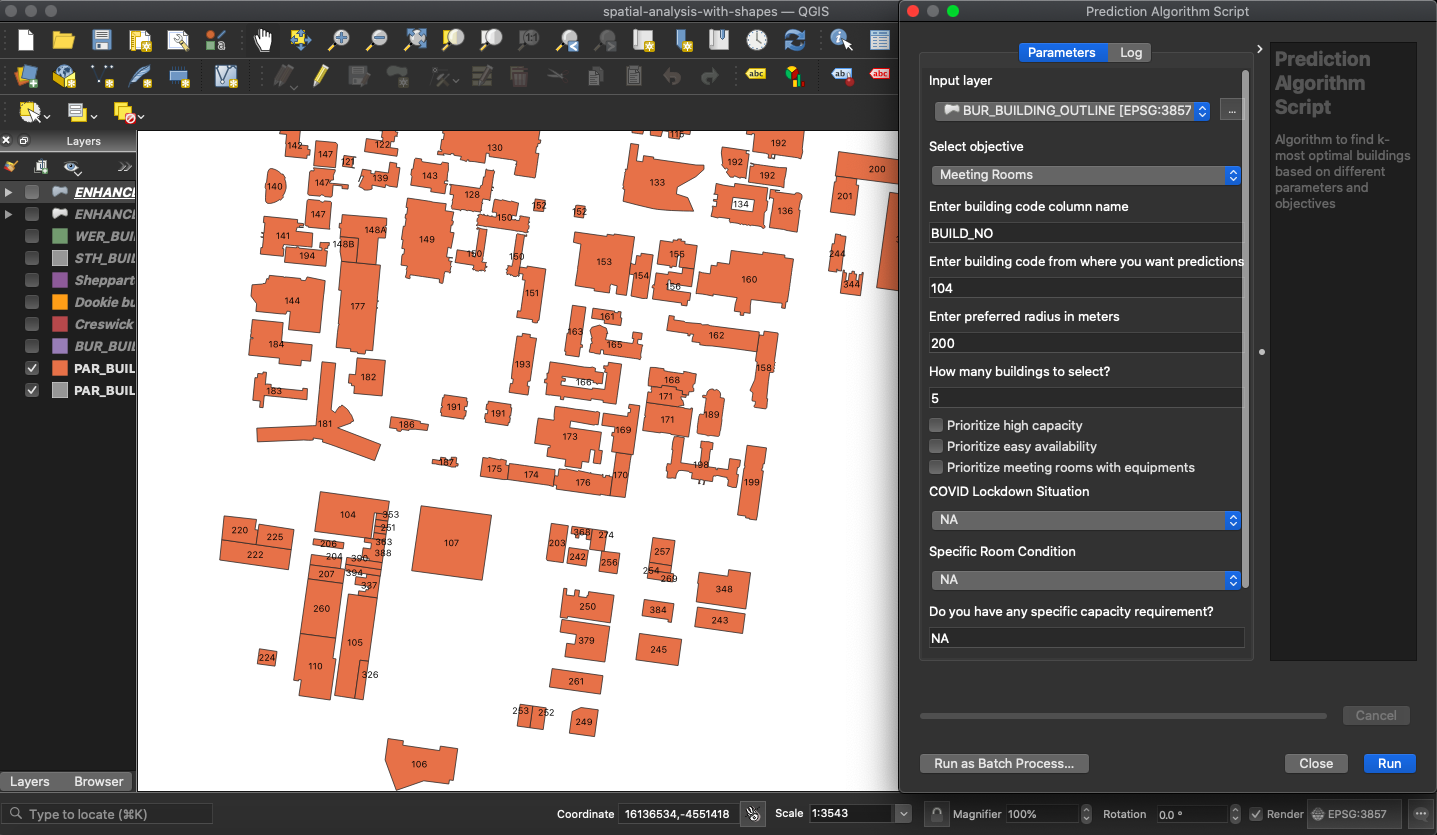
\includegraphics[width=16cm,keepaspectratio=true]{img14.png}
\caption{QGIS interface with map outline and prediction algorithm processing script}
\label{fig:img14}
\end{figure}

\subsubsection{Prerequisites}

In order to load and execute QGIS 3 python processing scripts, we need the following software installed in the machine:
\begin{itemize}
    \item \textbf{QGIS 3.14+}: We have tested our scripts on the QGIS 3.14 version so it is expected to run correctly on this version and above. This can be downloaded using URL: \url{https://qgis.org/en/site/forusers/download.html}.
    \item \textbf{Python 3+}: The scripts are implemented on python 3.6 version and it is expected to run correctly on the version above 3.6. This can be download using URL: \url{https://www.python.org/downloads/}.
\end{itemize}

\subsubsection{Installing required python packages \& configuring QGIS 3}

QGIS 3 installation comes with pyQGIS 3 which is already installed with the required libraries needed for executing our custom created processing scripts. Hence, other processing scripts can run without any installation, except \texttt{finding optimal radius script}. In order to execute our \texttt{finding optimal radius script} which is internally using the \texttt{sklearn k-means} algorithm, the package should be installed and connected with the QGIS space. This can be achieved using the following steps:

\begin{itemize}
    \item Step-1: First, we are required to install `sklearn` package in the python space. This can be achieved using the following command in the windows cmd or Linux/macOS terminal: \texttt{pip install -U scikit-learn} as shown below.
    
    \begin{figure}[H]
\centering
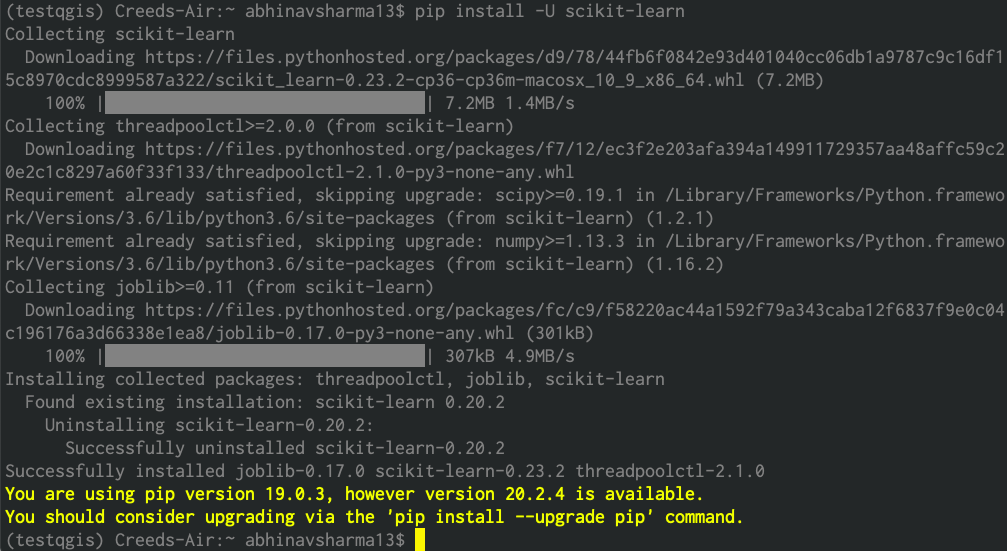
\includegraphics[width=10cm,keepaspectratio=true]{resources/images/installq1.png}
\caption{Step-1: Installing sklearn package}
\label{fig:installq1}
\end{figure}
    
    \item Step-2: After installation of the above package, we need to grab the site-packages path of the python. This can be achieved using the following command in windows cmd or Linux/macOS terminal: \texttt{python3 -m site} as shown below.
    
        \begin{figure}[H]
\centering
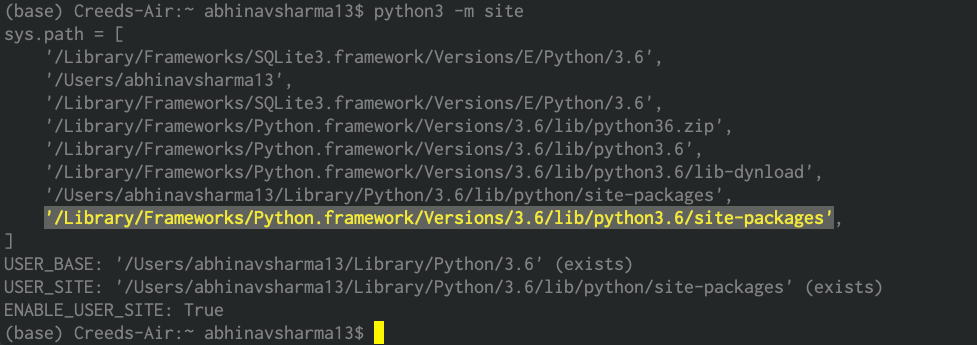
\includegraphics[width=10cm,keepaspectratio=true]{resources/images/installq2.png}
\caption{Step-2: Get python3 site-packages path}
\label{fig:installq2}
\end{figure}

    \item Step-3: After the site-packages location is found, we can open the QGIS 3 and go to preferences/settings to reach the environment section as shown below.
    
            \begin{figure}[H]
\centering
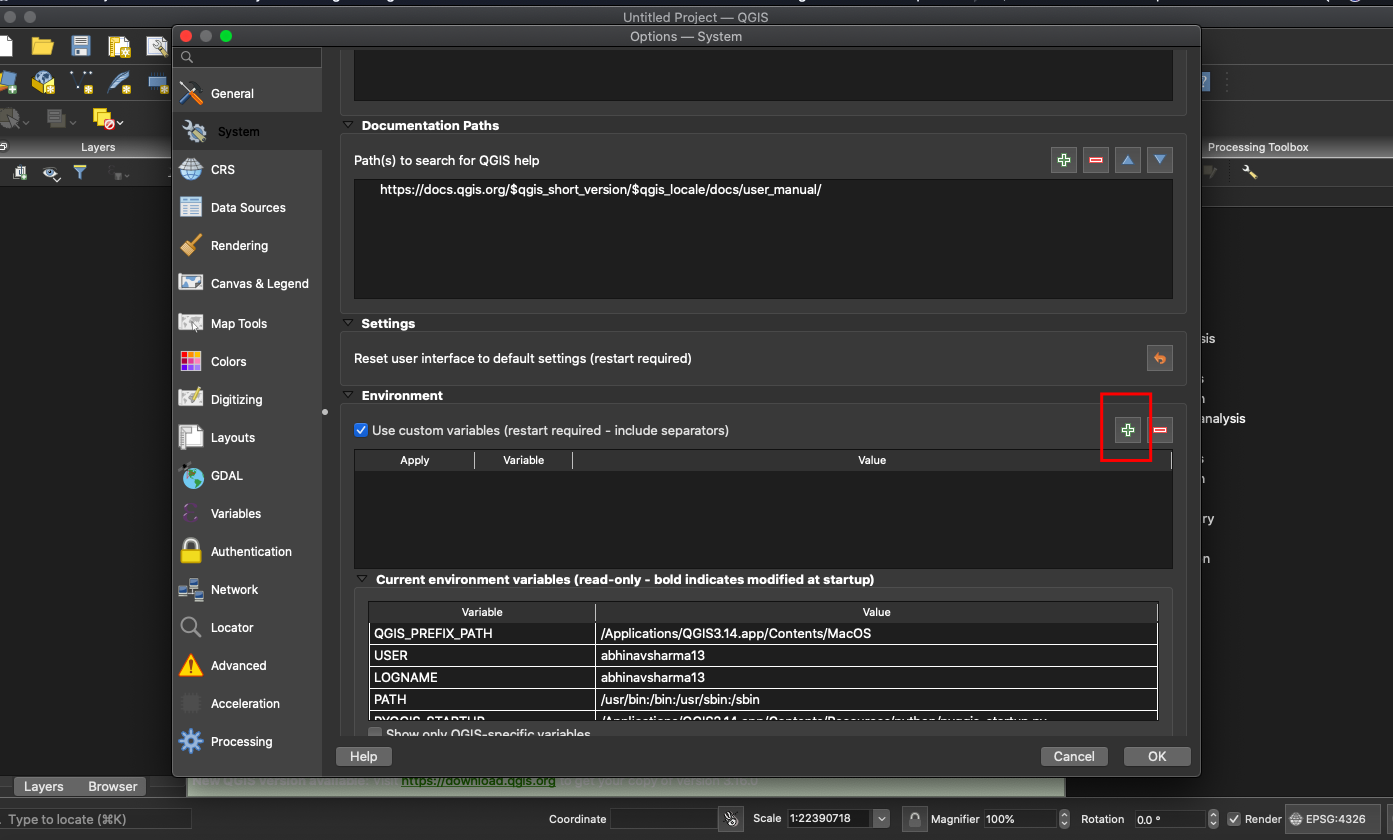
\includegraphics[width=12cm,keepaspectratio=true]{resources/images/installq3.png}
\caption{Step-3: Add custom environment}
\label{fig:installq3}
\end{figure}

\item Step-4: Finally, we will add the copied site package path as the custom environment in the QGIS space using \texttt{append} option on the \texttt{PYTHONPATH} variable as shown below.

            \begin{figure}[H]
\centering
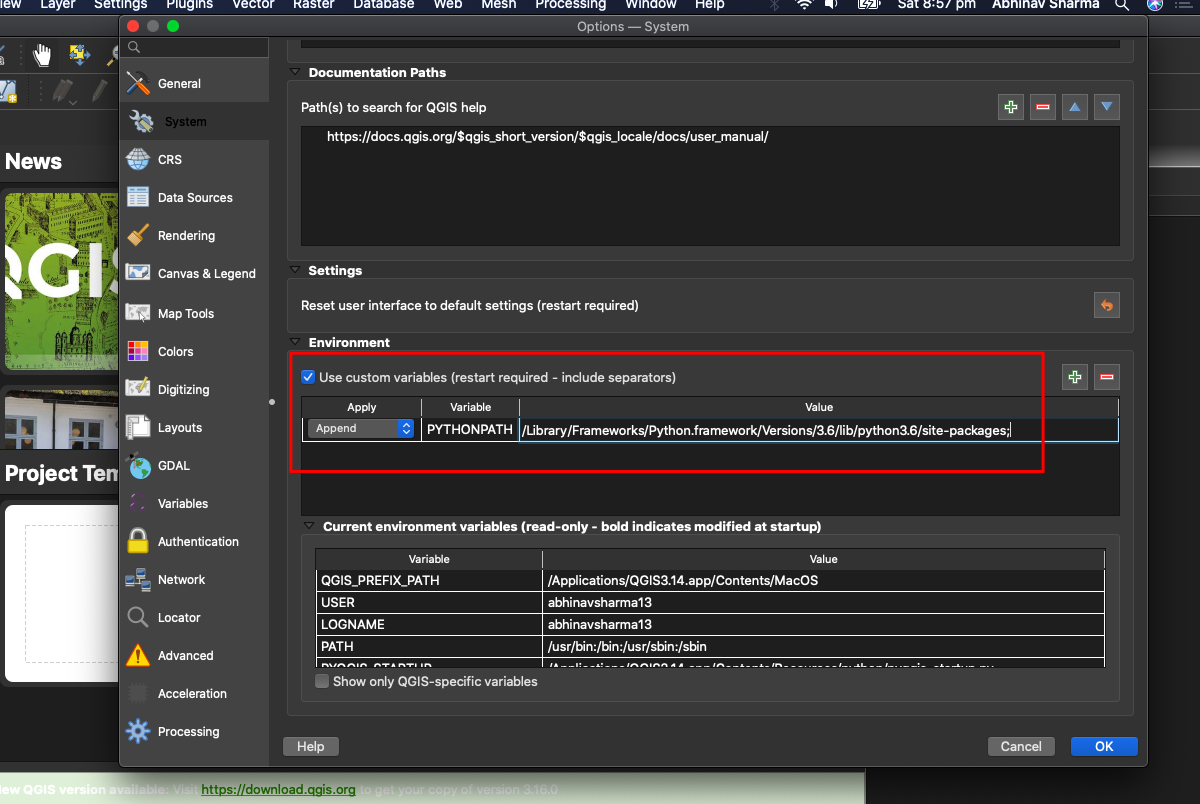
\includegraphics[width=12cm,keepaspectratio=true]{resources/images/installq4.png}
\caption{Step-4: Appending python site package path in the PYTHONPATH of QGIS 3}
\label{fig:installq4}
\end{figure}

\end{itemize}

These steps will effectively configure the QGIS 3 space to run all our custom python processing scripts without any errors or exceptions.
\pagebreak
\subsubsection{Executing QGIS data loader script}

QGIS process scripts can be accessed and loaded by following the below steps.

\begin{itemize}
    \item Step-1: Open the project and then click on the highlighted icon to open the processing script toolbox.
\begin{figure}[H]
\centering
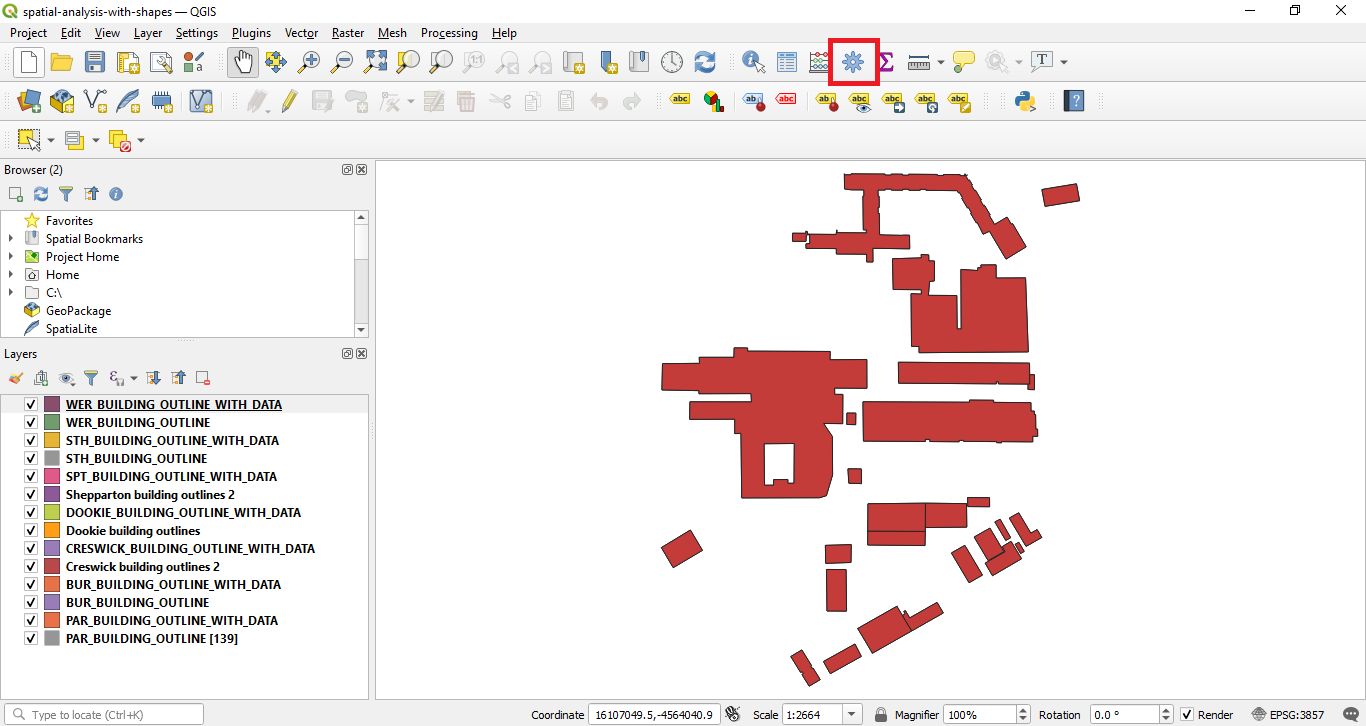
\includegraphics[width=12cm,keepaspectratio=true]{resources/step1.PNG}
\caption{Step-1: Accessing Python Process Toolbox of QGIS 3}
\label{fig:accesstoolbox}
\end{figure}
\item Step-2: Click on the highlighted icon and then click on \texttt{Add Script to toolbox}. To add the script to the processing toolbox.

\begin{figure}[H]
\centering
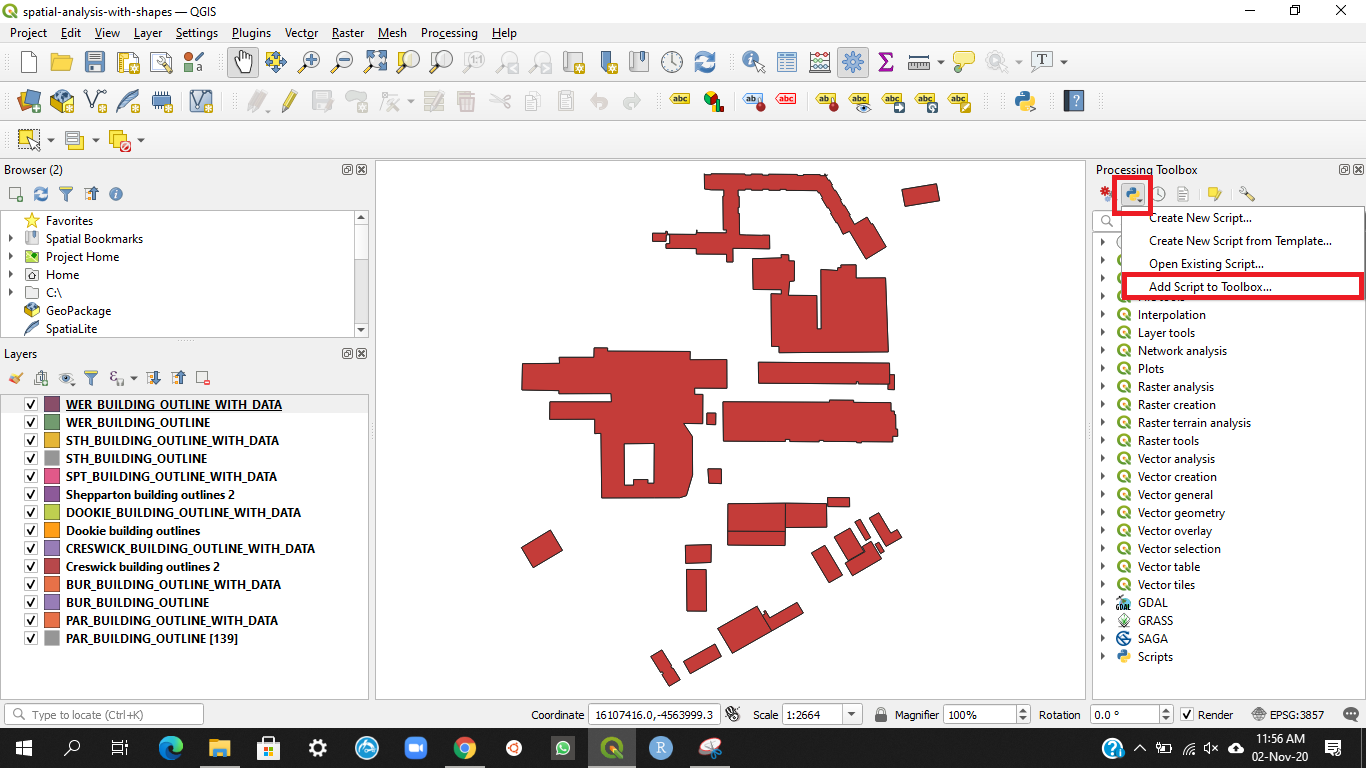
\includegraphics[width=12cm,keepaspectratio=true]{resources/step2.png}
\caption{Step-2: Adding Scripts to  Process Toolbox of QGIS 3}
\label{fig:addtotoolbox}
\end{figure}

\item Step-3: After clicking on the above option. Select a script file that you need to import, in this case, it would be \texttt{FINAL\_qgis\_data\_loader\_script}.

\begin{figure}[H]
\centering
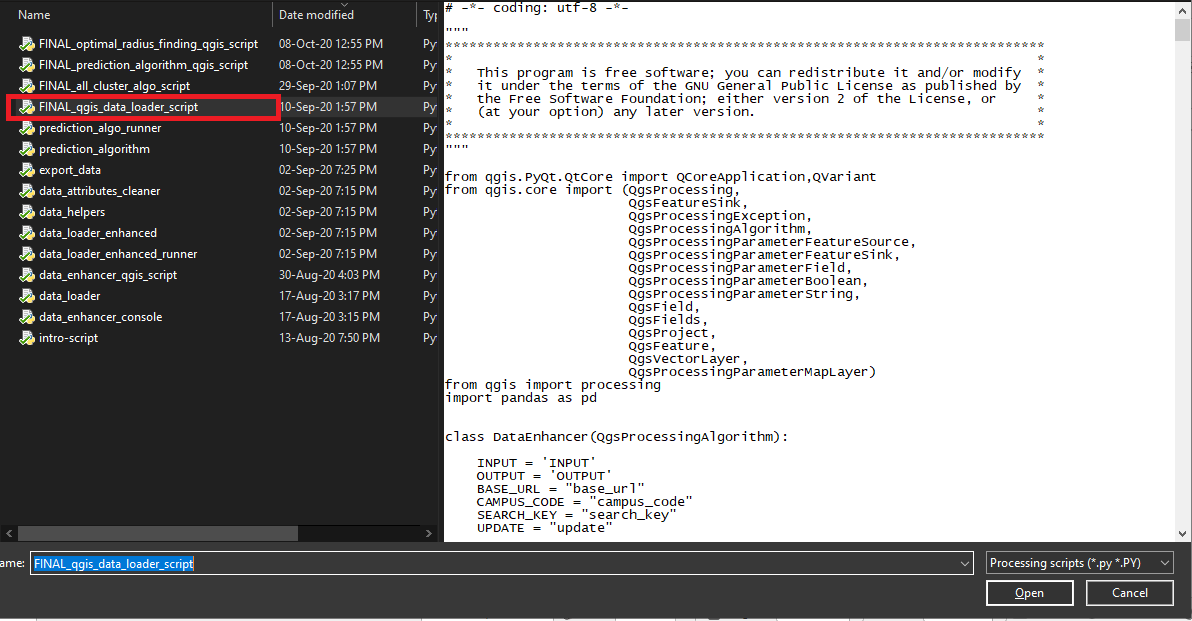
\includegraphics[width=12cm,keepaspectratio=true]{resources/step3.PNG}
\caption{Step-3: Select Scripts to  add to the Process Toolbox of QGIS 3}
\label{fig:selectscript}
\end{figure}

\item Step-4: Script will be added to the following directory in the processing toolbox.

\begin{figure}[H]
\centering
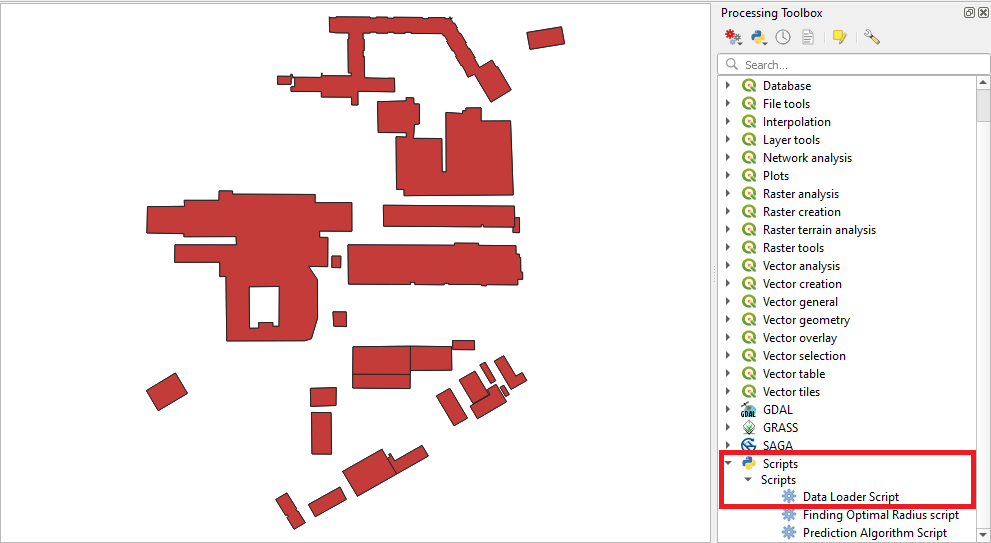
\includegraphics[width=12cm,keepaspectratio=true]{resources/step4.PNG}
\caption{Step-4: View Scripts added to the Process Toolbox of QGIS 3}
\label{fig:ads}
\end{figure}

\item Step-5: Right-click on the \texttt{Data Loader Script} and it will open a dialog box. Fill the information into the required fields. There is an option to update the base layer and not create the new layer, which can be selected as per the convenience and click on execute.

\begin{figure}[H]
\centering
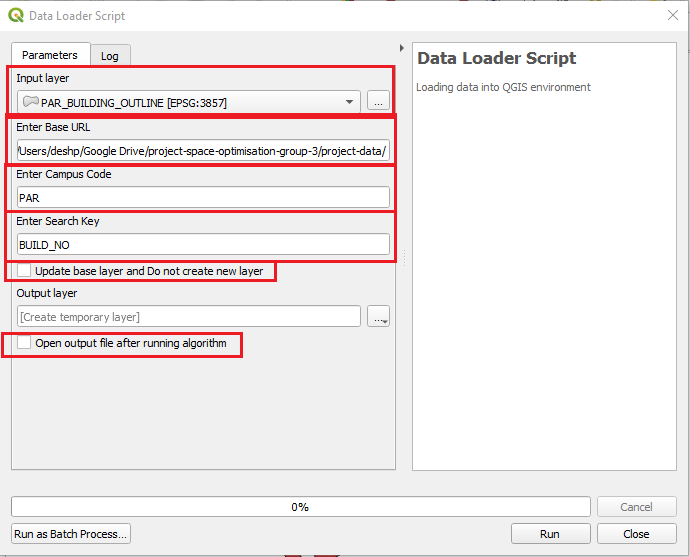
\includegraphics[width=12cm,keepaspectratio=true]{resources/dataloader.PNG}
\caption{Step-5: Execute Data Loader script in QGIS 3}
\label{fig:dls}
\end{figure}

\item Step-6: After clicking on \texttt{Run}, without selecting the \texttt{Update base layer and do not create new layer option}, the script will execute with the following logs.

\begin{figure}[H]
\centering
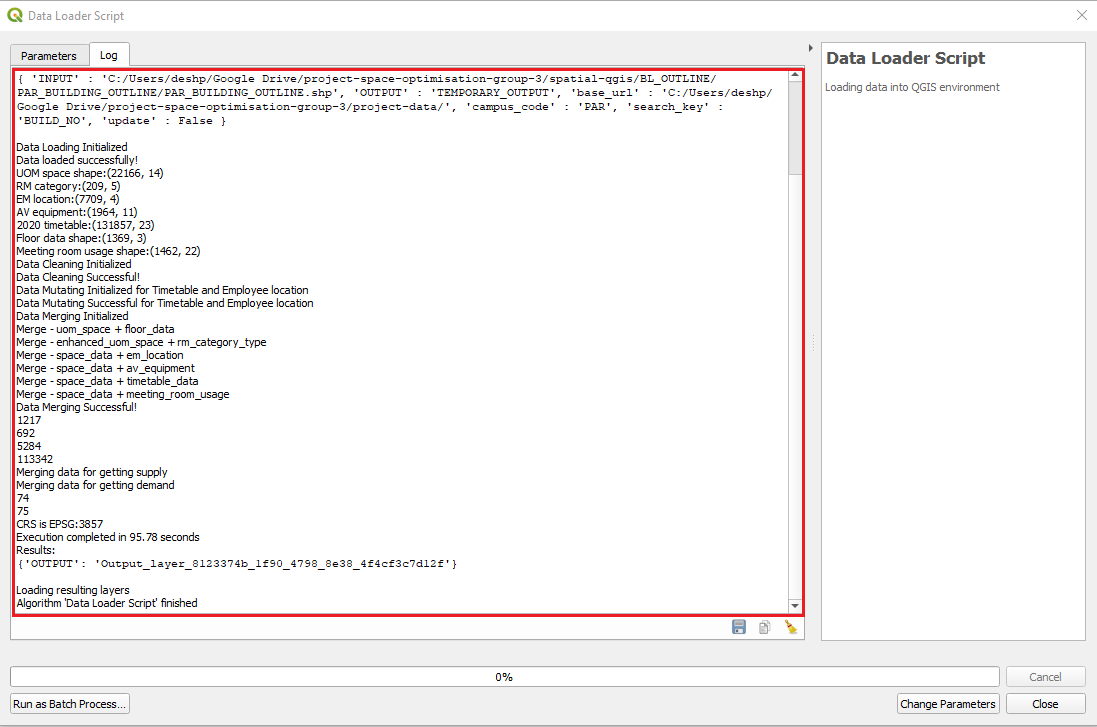
\includegraphics[width=12cm,keepaspectratio=true]{resources/dlexec.PNG}
\caption{Step-6: Logs after executing Data Loader script in QGIS 3}
\label{fig:dlsexec}
\end{figure}

\item Step-7: If the option \texttt{Update base layer and do not create new layer option} was selected, the script will stop with an error but the layer would be updated. An error was introduced to stop the script execution. The following figure shows the error message and execution of the script.
\begin{figure}[H]
\centering
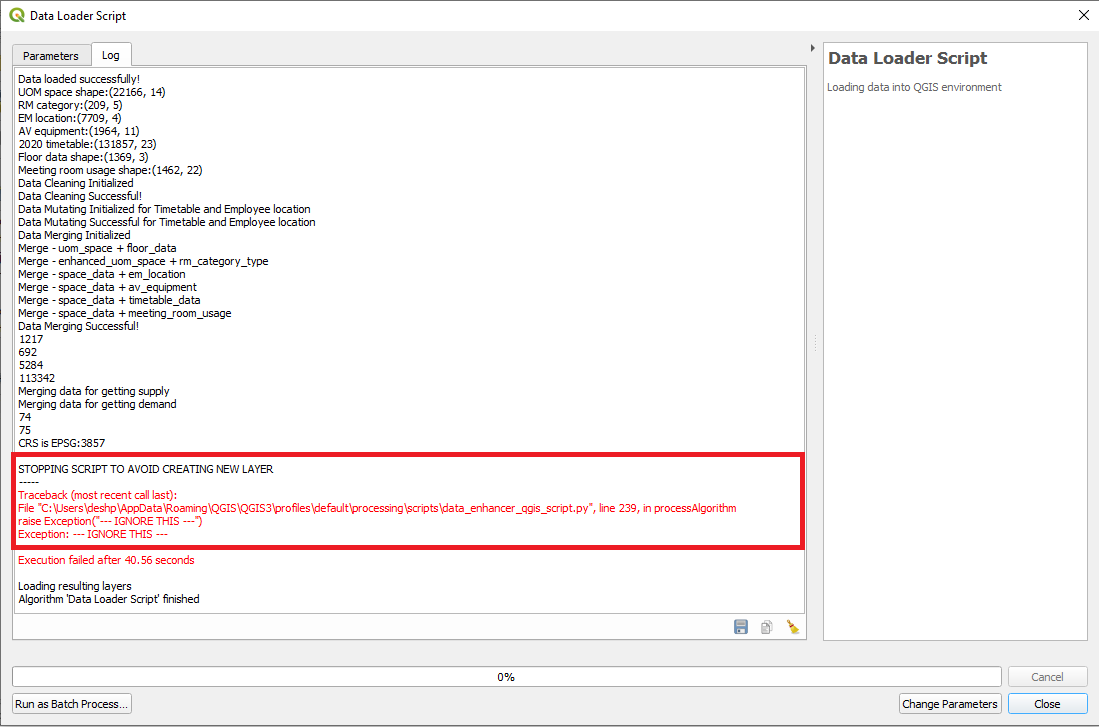
\includegraphics[width=12cm,keepaspectratio=true]{resources/update.PNG}
\caption{Step-7: Logs after executing Data Loader script with Base layer update in QGIS 3}
\label{fig:update}
\end{figure}
\end{itemize}

\subsubsection{Executing QGIS finding optimal radius script}
After loading the data into the QGIS environment, we need to use to calculate the optimal hyper-parameters (B and $\delta$). Following steps from step-2 to step-4 from the above process, you need to add \texttt{FINAL\_optimal\_radius\_finding\_qgis\_script}.

\begin{itemize}
    \item Step-1: After adding \texttt{FINAL\_optimal\_radius\_finding\_qgis\_script} to the toolbox. Right click on the highlighted script and click on execute.
    
\begin{figure}[H]
\centering
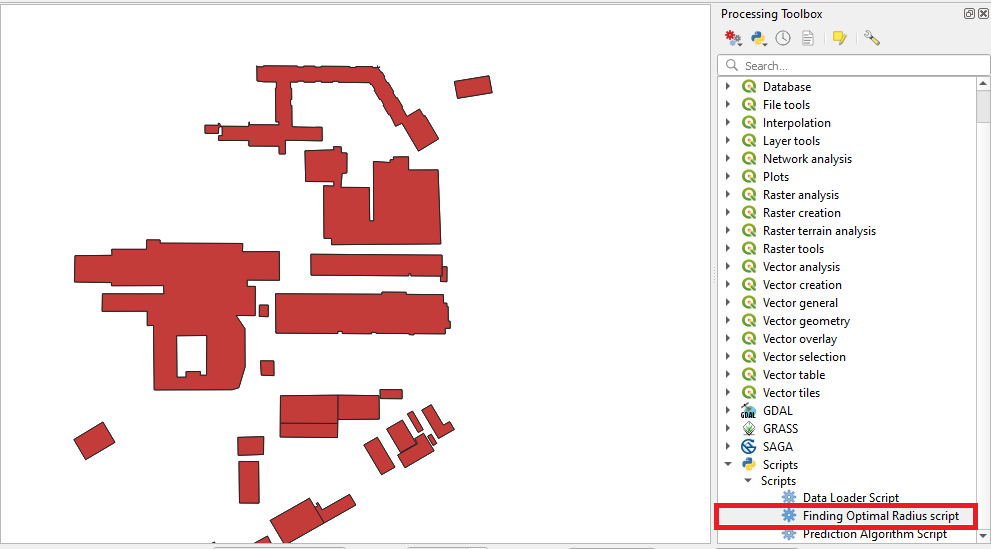
\includegraphics[width=12cm,keepaspectratio=true]{resources/opt1.PNG}
\caption{Step-1: Adding Optimal radius finding script in QGIS 3}
\label{fig:opt1}
\end{figure}
    
\item Step-2: A form will open, fill out all the details into the form,
select the input layer with all the enriched data from Data Loader, Select objective, Building Code Column Name, Building Code, Path to store plots, etc.

\begin{figure}[H]
\centering
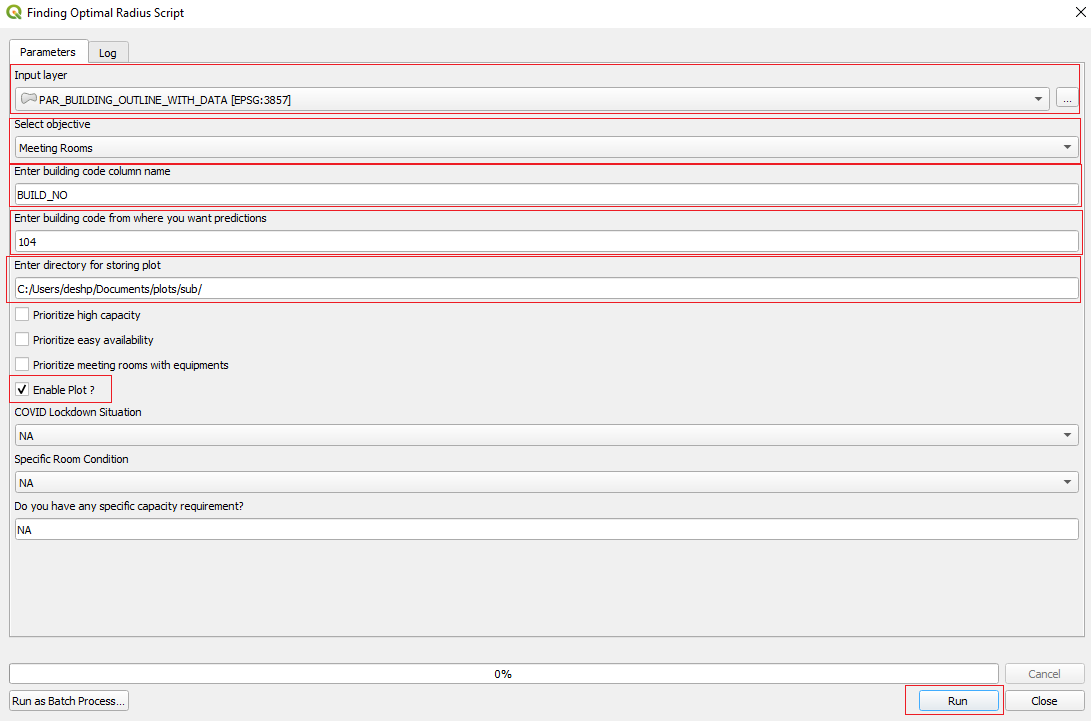
\includegraphics[width=12cm,keepaspectratio=true]{resources/opt2.PNG}
\caption{Step-2: Executing Optimal radius finding script in QGIS 3}
\label{fig:opt2}
\end{figure}

\item Step-3: After running the script, the following message appears in the logs. Giving the optimal radius and delta parameter.

\begin{figure}[H]
\centering
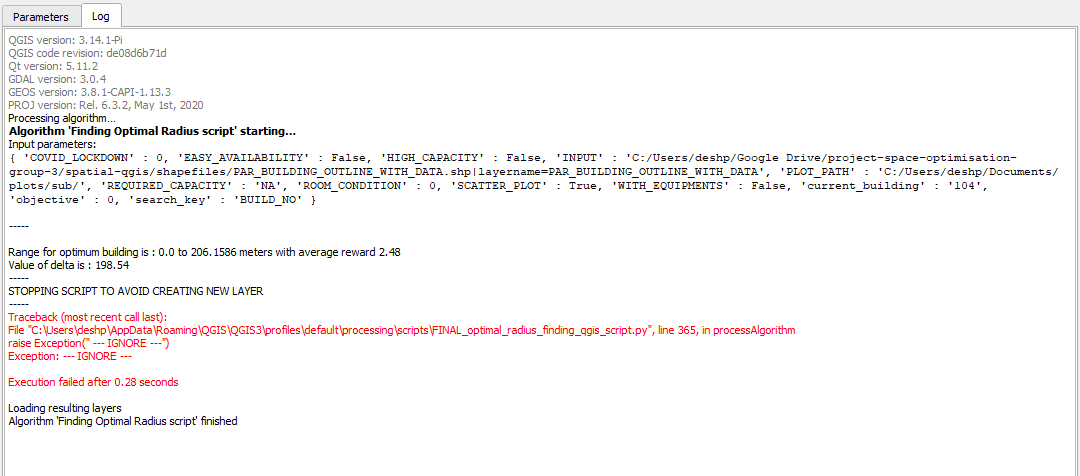
\includegraphics[width=12cm,keepaspectratio=true]{resources/opt3.PNG}
\caption{Step-3:Logs after executing Optimal radius finding script in QGIS 3}
\label{fig:opt3}
\end{figure}
\end{itemize}

\subsubsection{Executing QGIS prediction algorithm script}
After getting the values for both the constraints from the previous algorithm to find the rewarding buildings. Following steps from step-2 to step-4 from Data Loader steps, you need to add \texttt{FINAL\_prediction\_algorithm\_qgis\_script}.

\begin{itemize}
    \item Step-1: After adding \texttt{FINAL\_prediction\_algorithm\_qgis\_script} to the toolbox. Right click on the highlighted script and click on execute.

    
\begin{figure}[H]
\centering
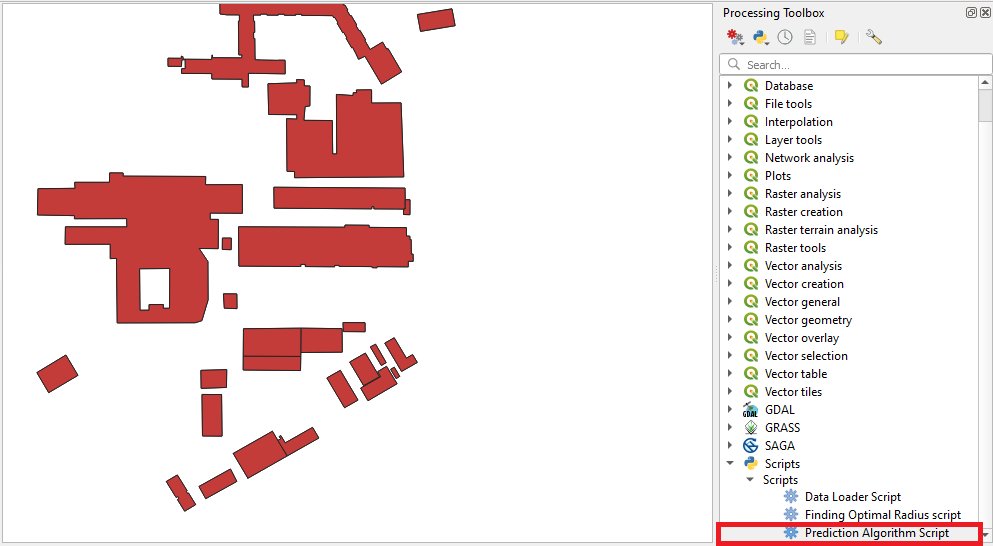
\includegraphics[width=12cm,keepaspectratio=true]{resources/p1.PNG}
\caption{Step-1: Adding Prediction Algorithm script in QGIS 3}
\label{fig:p1}
\end{figure}

\item Step-2: A form will open, fill out all the details into the form,
select the input layer with all the enriched data from Data Loader, Select objective, Building Code Column Name, Building Code, Path to store plots, etc. and use the values of \texttt{radius, delta} from the previous algorithm. Choose the same factors that were chosen to get the constraint values.

\begin{figure}[H]
\centering
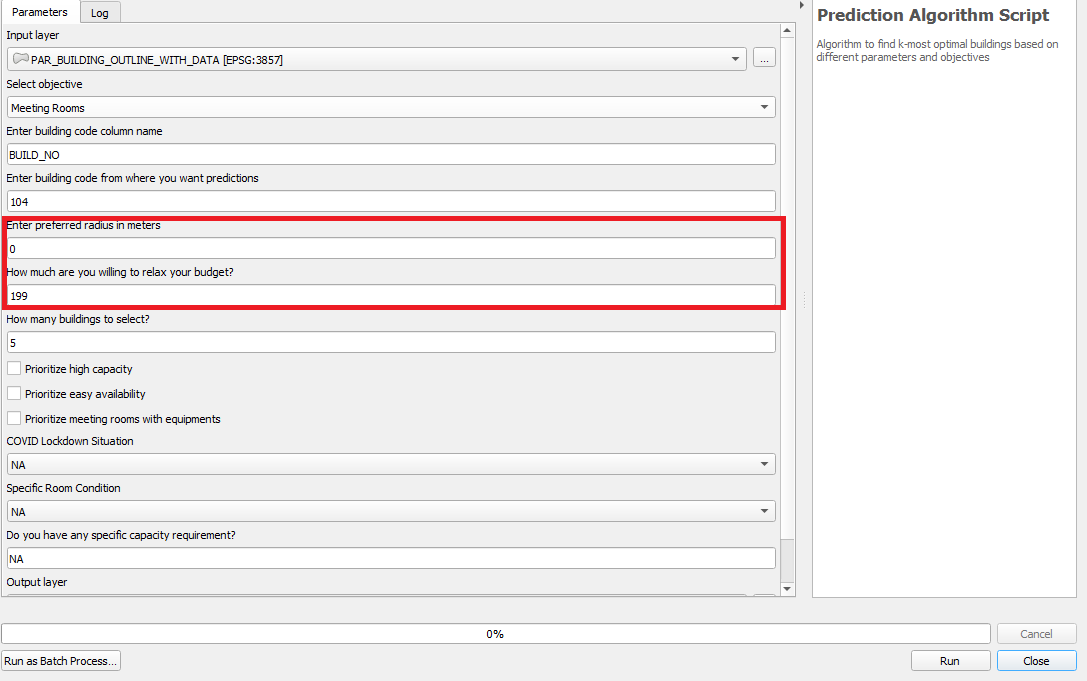
\includegraphics[width=12cm,keepaspectratio=true]{resources/p2.PNG}
\caption{Step-2: Executing Prediction Algorithm script in QGIS 3}
\label{fig:p2}
\end{figure}

\item Step-3: After running the script, the following message appears in the logs. The results of the top \texttt{k} buildings are displayed in the logs. Do not worry about the error message it is just to stop the execution of the script.

\begin{figure}[H]
\centering
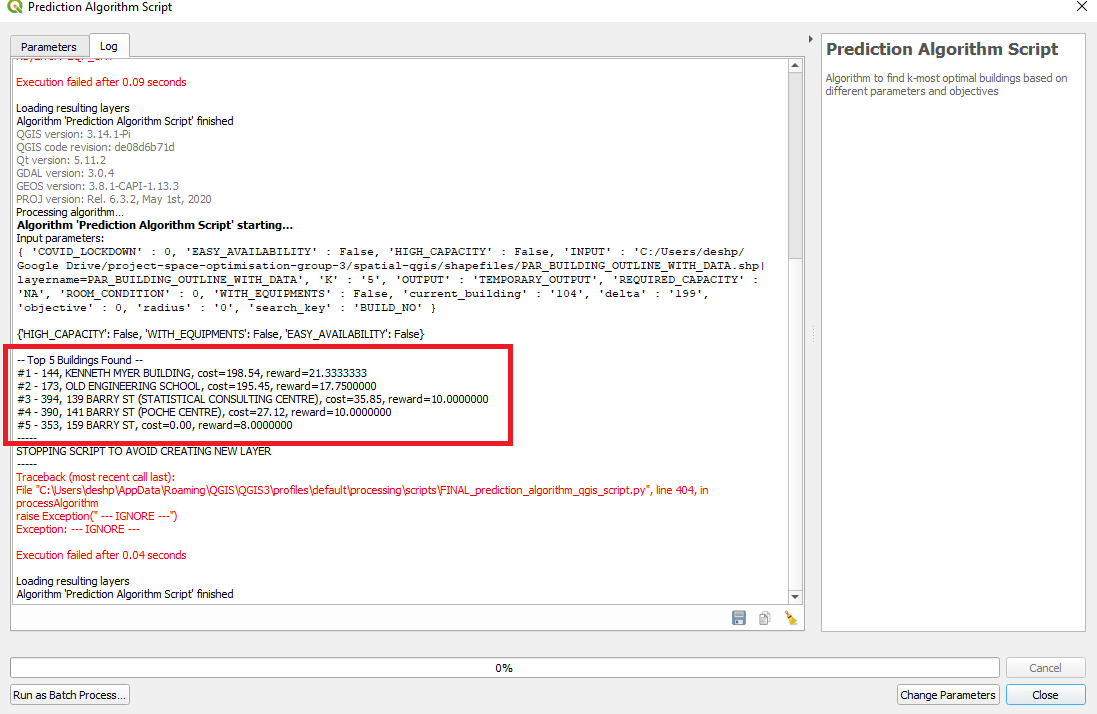
\includegraphics[width=12cm,keepaspectratio=true]{resources/p3.PNG}
\caption{Step-3: Logs after executing Prediction Algorithm script in QGIS 3}
\label{fig:p3}
\end{figure}
\end{itemize}

\subsection{Collected Results}

\subsubsection{Spatial Algorithm Results}
\import{content/results/spatial/}{appendix_meeting_rooms.tex}

\import{content/results/spatial/}{appendix_toilet_facilities.tex}

\subsubsection{Floor Algorithm Results}
\import{content/results/floors/}{appendix_meeting_rooms.tex}

\import{content/results/floors/}{appendix_toilet_facilities.tex}

\subsection{Research Paper} \label{rpaper}

\subsubsection{Searching k-Optimal Goals for an Orienteering Problem on a Specialized Graph with Budget Constraints}

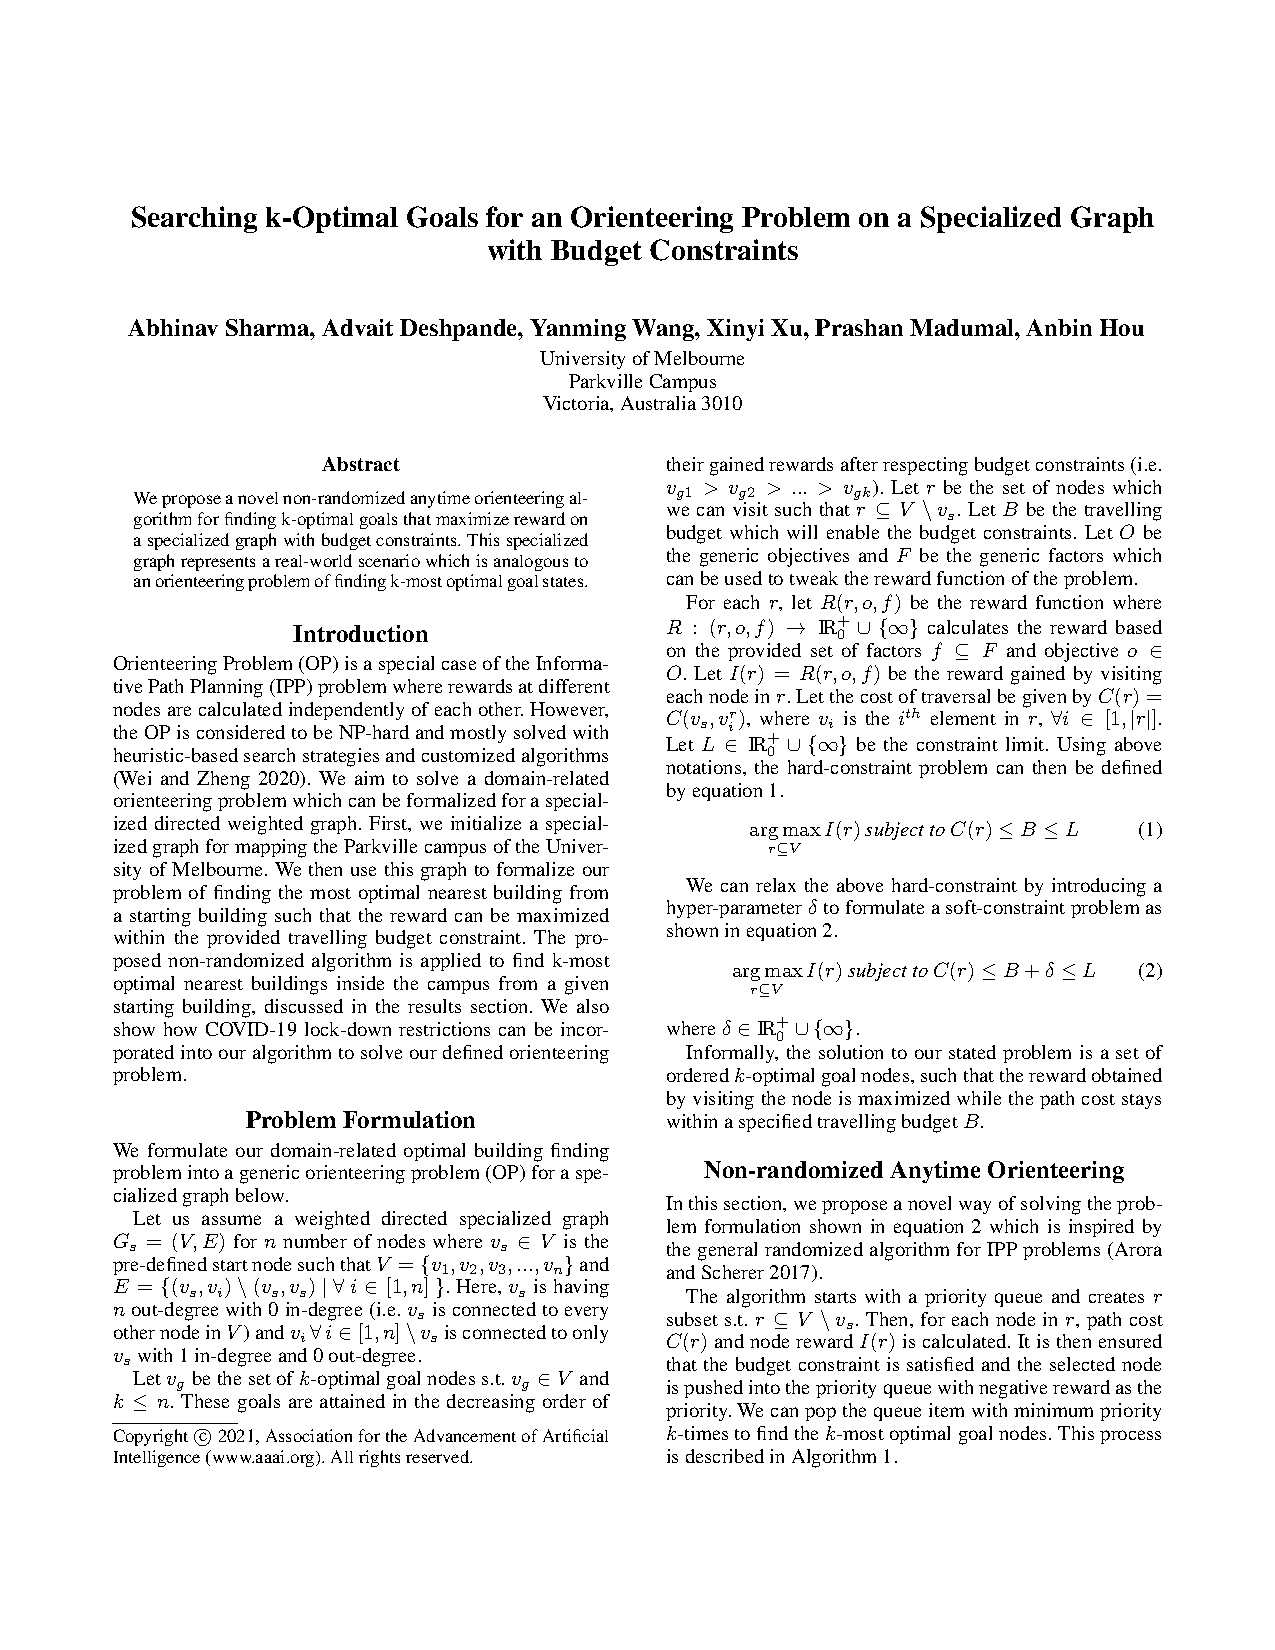
\includepdf[pages=-]{resources/paper}